\documentclass{../industrial-development}
\graphicspath{{09-software-project-management/}}

\title{Управление программными проектами}
\author{Мартынов Андрей Олегович, ИВТ--21 МО}
\date{}

\begin{document}

\begin{frame}
  \titlepage
\end{frame}

\section{Управление программными проектами}

\subsection{Основные понятия}

\begin{frame} \frametitle{Основные понятия}
	\begin{block}{Определение}
		\alert{Проект} --- временное предприятие, предназначенное для~создания уникальных продуктов, услуг или результатов
	\end{block}
	\begin{block}{Определение}
		\alert{Управление проектами} --- область деятельности, в ходе которой определяются и достигаются четкие цели проекта при балансировании между объёмом работ, ресурсами, временем, качеством и рисками
	\end{block}
\end{frame}
\lecturenotes
Программирование - это творческий процесс. И во все времена задача управления творчеством была актуальна. Инвесторам, менеджерам, государству хотелось бы иметь предсказуемость на счёт того, когда будет выпущен разрабатываемый творческий продукт (будь это книга, самолёт, компьютерная программа или фильм).

Творческая работа может вестись как индивидуально, так и коллективно. При этом в коллективе чаще всего присутствуют специалисты из разных областей (например художник, дизайнер и программист). Управление проектом подразумевает планирование, координацию и контроль работ по проекту для достижения его целей в рамках заданных сроков и бюджета.

\subsection{Параметры проекта}

\begin{frame} \frametitle{Параметры проекта}
	В проекте должны быть определены:
	\begin{itemize}
		\item Цели и результаты (область охвата)
		\item Уровень качества
		\item Этапы и сроки выполнения работ
		\item Бюджет
	\end{itemize}
\end{frame}
\lecturenotes
Перечисленные параметры проекта тесно связаны между собой. Область охвата, качество, время и стоимость тесно связаны между собой. Они образуют "треугольник проекта".

\subsection{Треугольник проекта}

\begin{frame} \frametitle{Треугольник проекта}
	\centerline{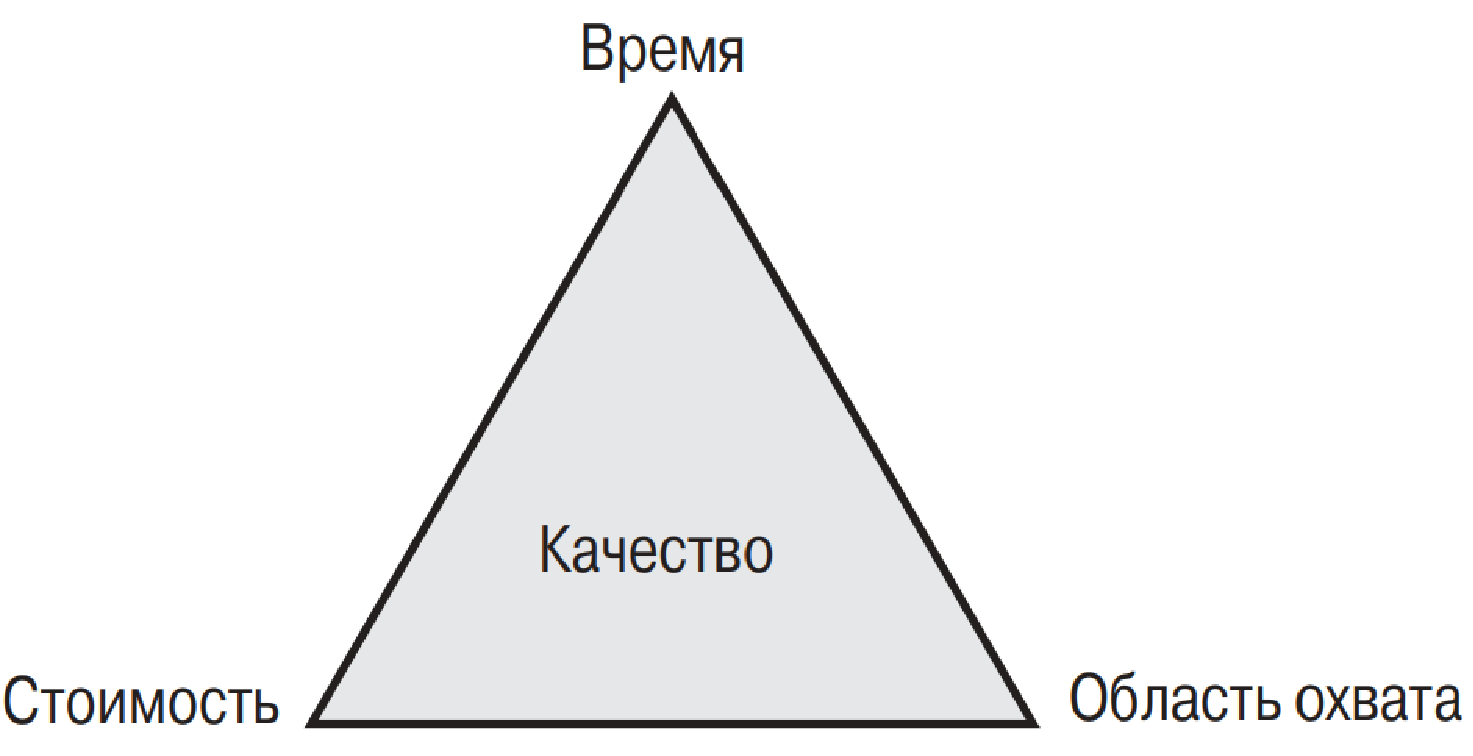
\includegraphics[width=0.8\textwidth]{trinagle.pdf}}
\end{frame}
\lecturenotes
Качество находится в цетре треугольника. Изменение любой из сторон треугольника неизбежно влечет за собой изменения других параметров проекта и оказывает влияние на качество. Увеличение области охвата может привести к увеличению времени. Дополнительное время позволит повысить качество отдельных работ и всего проекта. С другой стороны, увеличение времени или области охвата предполагает дополнительные расходы. Чтобы не допустить повышения стоимости проекта, приходится уменьшать область охвата или время (либо и то, и другое), но при этом возможно снижение качества.

\subsection{Параметры управления}

\begin{frame} \frametitle{Параметры управления}
	Параметами урпавления проекта являются:
	\begin{itemize}
	\item Сроки
	\item Объём проекта
	\item Объём работы
	\item Ценность проекта для потребителя
	\item Техническая и технологическая сложность
	\item Внешнее качество проекта
	\item Внутреннее качество проекта
	\item Риски
	\item Психологическое состояние команды
	\end{itemize}
\end{frame}

\subsection{Задачи управления}
\begin{frame} \frametitle{Задачи управления}
	Задачами управления проекта являются:
	\begin{itemize}
	\item Определение цели проекта
	\item Создание структуры проекта
	\item Определение необходимых объемов и источников финансирования
	\item Подбор команды исполнителей
	\item Определение сроков выполнения проекта
	\item Планирование и учет рисков
	\item Обеспечение контроля за ходом выполнения проекта
	\end{itemize}
\end{frame}

\subsection{Жизненный цикл проекта}

\begin{frame} \frametitle{Жизненный цикл проекта}
	\centerline{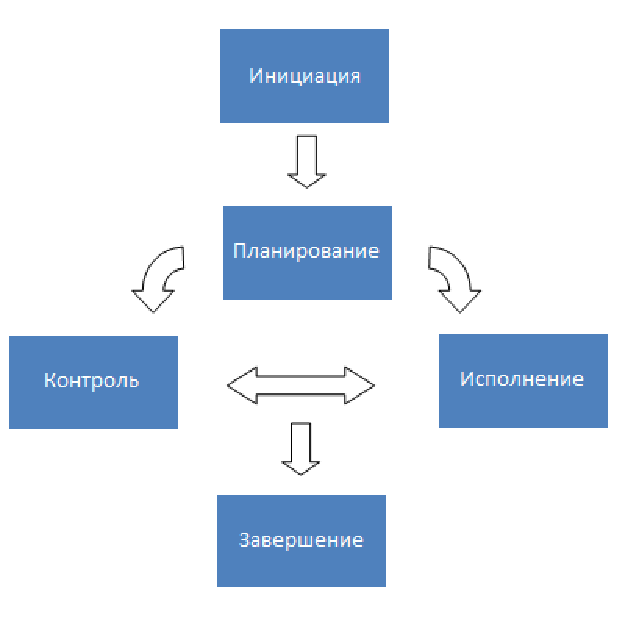
\includegraphics[width=0.7\textwidth]{manageproject.pdf}}
\end{frame}
\lecturenotes
Можно сказать, что любой проект начинается с формулировки и описания про
блемы. После того как проблема идентифицирована, формируется рабочая группа, основная задача которой – выявить одно или несколько решений данной проблемы. Для каждого решения определяются ресурсы и время, и на основании этих данных рассчитывается стоимость и оценивается степень риска. В процессе анализа проблемы выбирается наиболее приемлемое решение. С этого момента, собственно, и начинается разработка проекта, который должен будет реализовать выбранное решение.

\begin{frame} \frametitle{Инициация}
	\begin{block}{Назначение}
		Определяется суть проекта, его цель, заинтересованные в~нём лица. Чем меньше проект, тем проще эта стадия проходит
	\end{block}
	Этапы:
	\begin{itemize}
		\item Описание проблемы
		\item Определение требований
	\end{itemize}
\end{frame}
\lecturenotes
При разработке нового продукта первый этап (постановка задачи) лучше разбить на два – описание проблемы и определение требований. На этапе описания проблемы вместе с заказчиком определяются требования, которым должно соответствовать новое программное обеспечение. На этапе определения требований уточняются цели и требования, а также выполняется анализ рисков. Четкое представление конечных целей проекта на этапе определения требований уменьшает риски, связанные с ошибками в создаваемом проекте.

\begin{frame} \frametitle{Планирование}
	\begin{block}{Назначение}
		 Составляется список задач и мероприятий, которые должны быть выполнены в рамках проекта. Также указывается взаимосвязь между задачами и требующиеся ресурсы
	\end{block}
	Параллельно планированию обычно проводится оценка рисков и разрабатывается стратегия для их~предупреждения
\end{frame}
\lecturenotes
На этапе планирования окончательно определяются конечные цели проекта, составляется график работ, распределяются ресурсы, выполняется оценка времени, рассчитывается стоимость проекта. Параллельно проводится оценка рисков и разрабатывается стратегия действий для предупреждения рисков. В конце этапа планирования все участники проекта должны четко представлять, над чем именно они работают. Это поможет в дальнейшем на этапе реализации избежать разрастания масштаба проекта и тем самым сэкономить средства и время. Этап планирования завершается утвержде-
нием плана проекта, сметы и графика работ. Утвержденный план проекта называется контрольным или базовым.

\begin{frame} \frametitle{Исполнение и контроль}
	Исполнение и контроль проекта происходит циклами:
	\begin{itemize}
		\item Создание плана
		\item Реализация его части
		\item Контроль исполнения
		\item Внесение изменений в план
	\end{itemize}
\end{frame}
\lecturenotes
На данном этапе производится создание и тестирование продукта. Этап итеративен. Сначала ставится цель для текущей итерации и дата её завршения. Затем данную цель выполняют. В ходе выполнения цели ведётся контроль исполнения в процессе которого вносятся изменения в план проекта. После завершения итерации процесс повторяется до полного завершения проекта.

\section{Процессы управления программными проектами}

\begin{frame} \frametitle{Процессы управления}
	Основные процессы управления проектом:
	\begin{itemize}
		\item Управление задачами
		\item Управление сроками
		\item Управление качеством
		\item Управление рисками
	\end{itemize}
\end{frame}
\lecturenotes
Для контроля параметров используются процессы, каждый из которых сводится к определённому набору инструментов и процедур их применения. Рассмотрим основные процессы управления проектом

\subsection{Управление задачами}

\begin{frame} \frametitle{Управление задачами}
	\begin{block}{Назначение}
		Оценка объёма работы и распределение задач между сотрудниками
	\end{block}
	Цели системы контроля задач:
	\begin{itemize}
		\item Оценить и зафиксировать объём работы
		\item Распределить задачи между исполнителями
		\item Найти зависимости между различными задачами
		\item Определить, какие задачи заблокированы по тем или~иным причинам
	\end{itemize}
\end{frame}
\lecturenotes
Назначение управления задачами - оценка объёма работ и распределение задач между сотрудниками.
Цели:
1. Оценка и фиксация объёма работ
Сотрудники не должны выдумывать себе занятия, а заниматься задачами из заранее утверждённого списка.

2. Распределить задачи между работниками.
Необходимо убедиться, что у каждого работника имеется задача, и ни один из них не простаивает.

Пример. Если вы когда-нибудь наблюдали, как происходит починка аварии на теплотрассе, то наверняка замечали, что копает яму один рабочий, а вокруг него 10 человек стоят и смотрят, как он работает.

Следует также убедиться, что сотрудники не пренебрегают одними задачами в ущерб другим.

Пример. В гипермаркете продавцы отдела сантехники предпочитают находиться рядом с дорогими товарами, потому что премия за продажу дорогого оборудования получается выше. Как результат, если Покупатель хочет приобрести расходные материалы, то ему не с кем проконсультироваться. Так продавцы выполняют одни задачи и игнорируют другие. Получается, что сотрудники сами себе ставят или выбирают задачи, которые им больше нравятся.

3. Найти зависимости между различными задачами.
Задача обязательно должна быть согласована с задачами других сотрудников, всего проекта или его части. Продолжая пример с рабочим: может оказаться так, что рабочий выкопал яму, получил деньги, все 10 «начальников» отчитались, а на другой день пришёл приказ яму срочно закопать, потому что по этой дороге поедет президент. Об этом знали давно, просто «забыли» предупредить. А те, кто копал, не уточнили параметры своей задачи или рабочий вырыл одну яму, а надо было рыть чуть шире или чуть глубже или вообще в другом месте. То есть задача, может, и актуальна, но, при этом, не согласована или не точна.

4. Определить, какие задачи заблокированы по тем или иным причинам. 

Задачи могут быть заблокированы другими задачами. Пример задачи "Добавить выпадающий список для поиска перекрёстков". Эта задача не может быть выполнена пока не выполнена другая задача "Добавить экран поиска перекрёстков". В результате, сотрудник с заблокированной задачей может простаивать и терять время.

\begin{frame} \frametitle{Система контроля задач}
	\centerline{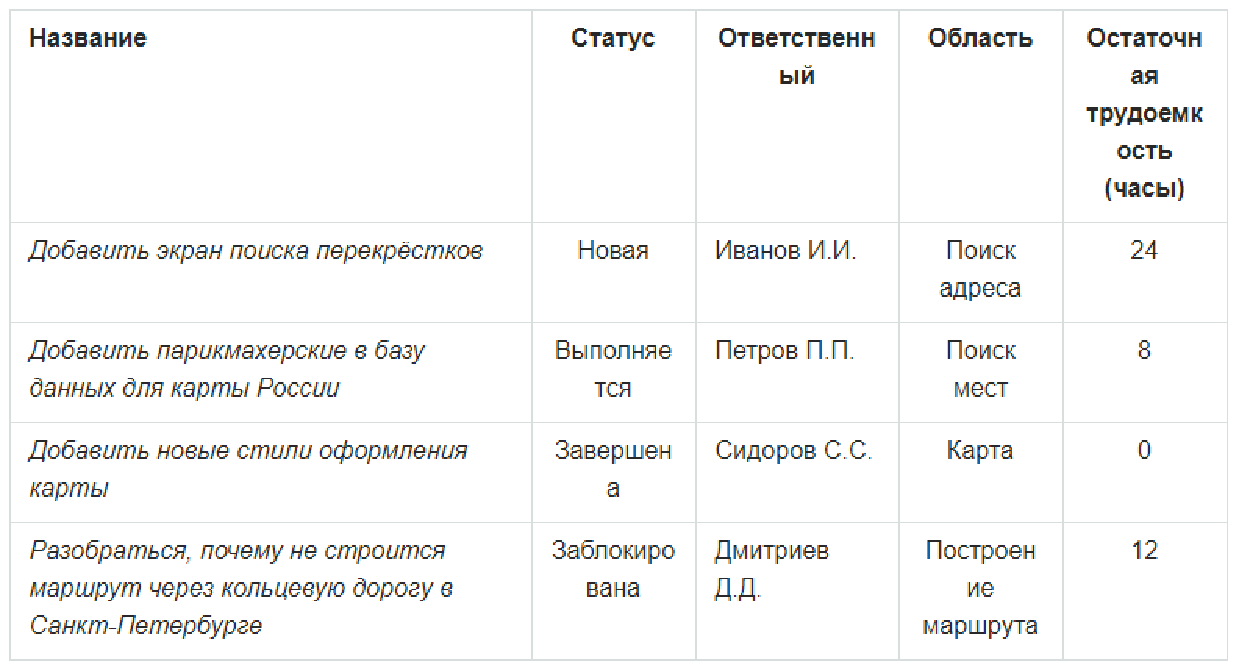
\includegraphics[width=1\textwidth]{gpstable.pdf}}
\end{frame}
\lecturenotes
Для управления задачами применяются системы контроля задач. Это основной инструмент работы над проектами и в небольших стартапах, и в крупных компаниях. Без системы контроля задач сложно представить работу любой команды, даже если команда состоит из одного исполнителя. Простейщая система контроля задач может быть представлена в виде обычной таблицы.
Название описывает в краткой форме суть вносимых изменений. В идеальном случае оно должно содержать проверяемый критерий, по которому можно судить о том, выполнена задача или нет.
Пример:
Добавить экран поиска перекрёстков. (Проверяемый критерий – экран. Он либо есть, либо его нет.)
Название задачи может включать в себя и название области программы (подсистемы), к которой относится задача. Это помогает при беглом взгляде на задачу понять, какому специалисту её следует поручить.
Пример:
1) Базы данных - Поиск мест
2) Интерфейс - Карты
Подсистему можно вынести в отдельную графу. Это позволит оценить объём работы, относящийся к той или иной части программы. Далее приведена круговая диаграмма объёма работ по подсистемам.

\begin{frame} \frametitle{Система контроля задач}
	\centerline{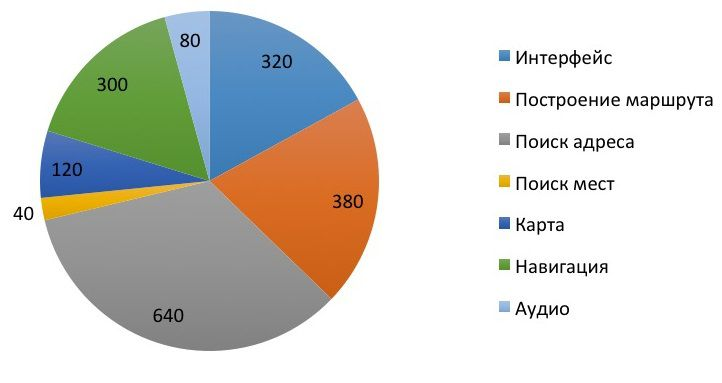
\includegraphics[width=1\textwidth]{circle.pdf}}
\end{frame}

\begin{frame} \frametitle{Использование системы контроля~задач}
	\begin{block}{}
		Первоначально задачи вносятся в систему контроля задач на этапе планирования проекта
	\end{block}
	Популярные системы контроля задач:
	\begin{itemize}
		\item Электронные таблицы Excel или Google Docs
		\item Redmine
		\item Jira
		\item BugZilla
		\item DropTask
		\item Hansoft
	\end{itemize}
\end{frame}
\lecturenotes
Первоначально задачи вносятся в систему контроля задач на этапе планирования проекта. Основная трудность заключается в том, что достаточно сложно предусмотреть все задачи и точно оценить время, которое займёт их выполнение.

Работу над проектом рекомендуется вести итеративно – двухнедельными или недельными итерациями. (Итеративность помогает быстро сделать некоторый законченный кусок работы и оперативно получить обратную связь.) В начале каждой итерации выполняется детальное планирование, в результате которого осуществляется выбор задач на итерацию. Если необходимо, то задачи детализируются, а их формулировки и оценки – уточняются.

Для управления задачами можно использовать готовые бесплатные или недорогие системы контроля задач перечисленные в слайде.
Любая сложная, и дорогая система управления проектом может быть заменена симбиозом Redmine и Google Docs.

\subsection{Управление сроками}

\begin{frame} \frametitle{Управление сроками}
	\begin{block}{Назначение}
		Оценка и контроль сроков реализации проекта
	\end{block}
	Цели управления сроками:
	\begin{itemize}
		\item Оценить текущий остаточный объём работы
		\item Определить величину отставания от плана
		\item Оценить прогресс каждого сотрудника и всей команды
	\end{itemize}
\end{frame}
\lecturenotes
Управление сроками нужно для оценки и контроля сроков реализации проекта. Цели включают в себя: определение текущего объёма работ, определение велечины отставания от плана, оценку програсса.

\begin{frame} \frametitle{Диаграмма сгорания задач}
	Прогресс работы сотрудника (реальный и~прогнозируемый):
	\centerline{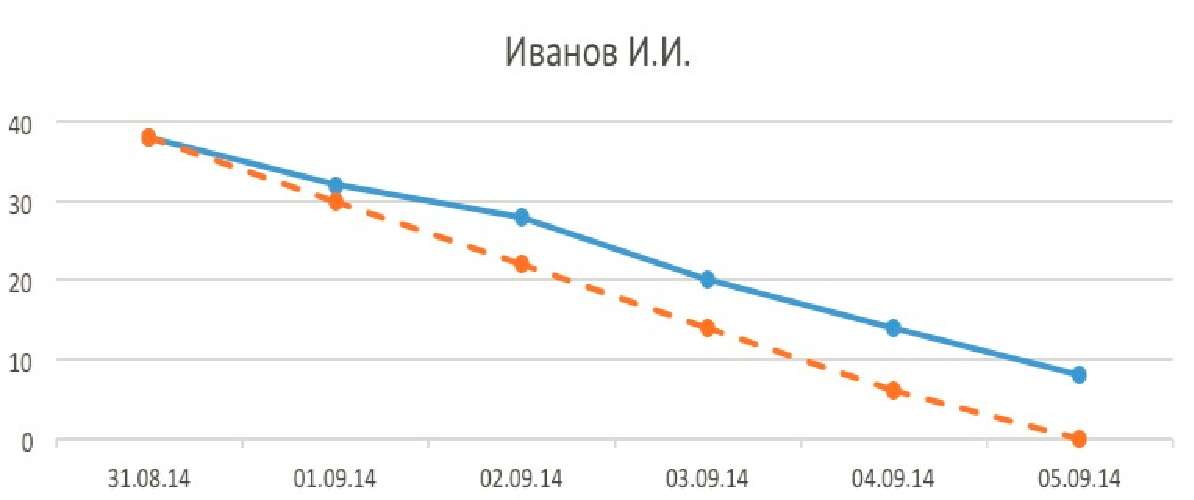
\includegraphics[width=1\textwidth]{ivanov.pdf}}
\end{frame}
\lecturenotes
Часто для управления сроками используется диаграмма сгорания. 

Диаграмма представляет собой две кривые. Одна из них (нарисованная пунктиром) показывает запланированное уменьшение объёма работы, т.е. то, как должно быть. Вторая кривая (нарисованная сплошной линией) представляет собой реальное изменение объёма работы. Каждая точка на этих кривых – это запланированный либо реальный объём работы, который остался на конец дня.

Кривые строятся как для каждого работника индивидуально, так и для всей команды в целом.

В конце каждого рабочего дня данные – объём оставшейся работы в часах – заносятся в таблицу. Данные берутся из графы «Остаточная трудоёмкость» таблицы задач.

Причины увеличения сроков задач анализируются и впоследствии заносятся в специальную базу знаний компании.

\begin{frame} \frametitle{Диаграмма Гантта}
	\centerline{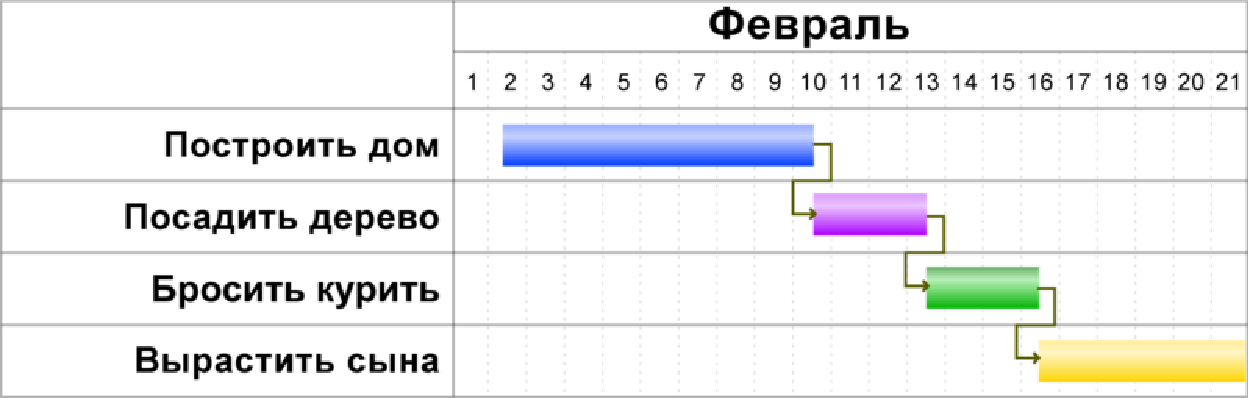
\includegraphics[width=1\textwidth]{gantt.pdf}}
\end{frame}
\lecturenotes
Диаграммы Ганта в наше время являются стандартом в управлении проектами, принципы которых используют как в теории, так и в практике.
В эру научного менеджмента Генри Гант создал инструмент, который показывает прогресс проекта в специальной диаграмме. Изначально диаграмма создавалась для отслеживания процесса построения кораблей. Сегодня же этот инструмент представляет собой горизонтальную столбчатую диаграмму для управления проектами.
Горизонтальная ось в диаграмме Ганта — шкала времени, которая может быть выражена в абсолютном значении либо значении времени, привязанного к началу проекта. Выбор времени зависит от типа проекта: обычно используются недели или месяцы. Столбы в диаграмме показывают время начала и окончания индивидуальной задачи в проекте.
Для больших проектов, задачи могут быть разделены на подзадачи, которые имеют собственные дополнительные диаграммы Ганта для более удобного прочтения.

\subsection{Управление качеством}

\begin{frame} \frametitle{Управление качеством продукта}
	\begin{block}{Назначение}
		Обеспечение надлежащего качества продукта
	\end{block}
	Цели
	\begin{itemize}
		\item Оценка сложности проекта
		\item Оценка ресурсов, необходимых на доводку качества
	\end{itemize}
\end{frame}
\lecturenotes
Крупные корпорации планируют качество продукта до начала разработки. Они не только прогнозируют количество дефектов, которое будет найдено в процессе работы над проектом, но и количество дефектов, которое так и не будет исправлено.

Пример. В одном из проектов было найдено 30 тысяч дефектов. Из них 15\% так и не было исправлено. Не смотря на то, что это некритические или очень редко встречающиеся ошибки, тем не менее, можно сказать, что приложение было выпущено с 4 500 ошибками.

Если приложение выпускается на регулярной основе (например, каждый год – новая версия), то прогноз разумно основывать на исторических данных. Его можно представить в виде таблицы, в которой приводится статистика по предыдущим версиям и прогнозные показатели для новой версии.

\begin{frame} \frametitle{Управление качеством продукта}
	Прогноз количества дефектов для мобильной навигационной системы GPS:
	\centerline{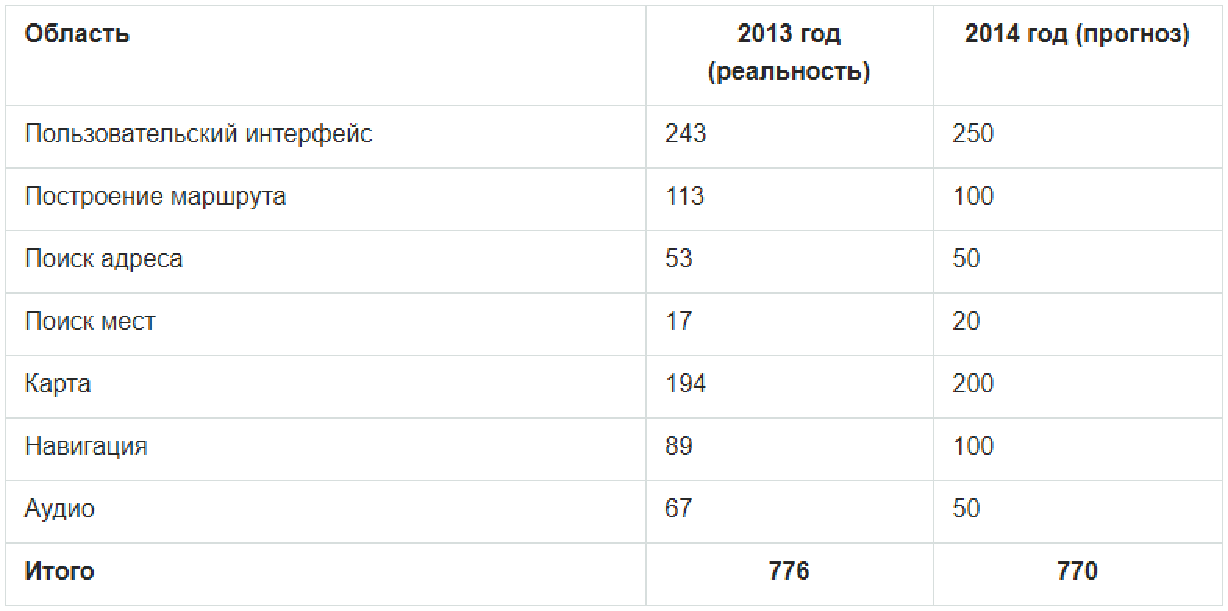
\includegraphics[width=1\textwidth]{gpstable1.pdf}}
\end{frame}
\lecturenotes
При старте проекта отдел контроля качества создаёт прогноз по багам. Во внимание принимаются исторические данные, прогнозируемый объём работы, сложность требований к новой версии приложения, а также опытность самой команды.

Прогноз даётся с разбивкой по подсистемам. Для увеличения точности используются две разные модели. Первая модель предусматривает дробление программы на подсистемы на основании различных технических критериев.

Например:
Пользовательский интерфейс
База данных
Аудио
Алгоритмы

Вторая модель предусматривает деление программы на подсистемы по пользовательским функциям.

Например:
Рисование карты
Построение маршрута
Навигация
Поиск адреса

Разные модели прогноза дополняют и проверяют друг друга.

Прогноз количества дефектов – не простая формальность, а серьёзный инструмент для планирования работы. Он помогает определить количество инженеров по качеству, которое собираются привлечь на проект. Прогноз также позволяет подсчитать время, необходимое для стабилизации программы.

Прогноз количества дефектов – достаточно консервативный инструмент. Менеджмент пересматривает его очень неохотно, потому что любой его пересмотр в сторону снижения может привести к тому, что трудновоспроизводимые ошибки не будут искаться. Предполагается, что в отсутствии надлежащего эталона, инженеры по качеству просто расслабятся и будут выполнять свою работу хуже, чем могли бы это делать.

\subsection{Управление рисками}
\begin{frame} \frametitle{Управление рисками}
	\begin{block}{Назначение}
		Предусмотреть риски, которые могут осложнить или сорвать проект, разработать план действий на случай срабатывания риска для нейтрализации его последствий
	\end{block}
	Цели:
	\begin{itemize}
		\item Описать выявленные риски
		\item Оценить важность каждого риска и вероятность его срабатывания
		\item Предложить план действия на случай того, если риск сработает
		\item Распределить риски между ответственными за их~устранение
	\end{itemize}
\end{frame}
\lecturenotes
Управление рисками похоже на анализ видов и последствий отказов: выявляются риски, оценивается их негативное влияние на проект, находятся решения для нейтрализации негативных последствий.

Цели управления рисками:
1. Описать выявленные риски.
Одна из характерных проблем в ряде компаний – люди не делятся опытом. Не происходит обмен информации по поводу типовых ошибок, рисков, решений. Необходимо делать информацию доступной для всей компании.
Нужно описывать решение сразу (по-возможности, следует находить идеальные решения). Т.е. выявить риск мало – надо сразу думать о том, как его предотвратить. Иначе риски так и остаются «граблями».

2. Оценить важность каждого риска и вероятность его срабатывания.
Пример. Риск того, что проект закроется из-за попадания метеорита в офис компании, обладает высокой важностью. Тем не менее, вероятность его срабатывания настолько низка, что безболезненно позволяет этот риск игнорировать.

3. Предложить план действия на случай того, если риск сработает.
Пример. При создании одной игры для маленьких девочек был серьёзный риск не уложиться в отведённые сроки. Было несколько причин у этого риска: новая команда, незнакомая платформа, для которой велась разработка, отсутствие отлаженной технологической инфраструктуры. Чтобы снизить риск, было принято решение организовать игру в виде последовательности мини-игр. Каждая такая игра была достаточно простой, не слишком сильно насыщенной графикой и другими персонажами. Кроме того, игрок был лишён свободы передвижения, т.е. мог двигаться только в заранее определённых направлениях. Это настолько упростило процесс разработки, что одна мини-игра в финальном качестве создавалась за 5 человеко-дней (имеется в виду работа инженера без учёта работы художника).

4. Распределить риски между ответственными за их устранение.
При ограниченных ресурсах в первую очередь следует уделять внимание рискам с наибольшим весом.
При описании риска также следует добавить план действий на случай его срабатывания или для уменьшения вероятности его срабатывания и/или его важности. Для каждого риска назначается ответственный, который отвечает за его нейтрализацию.

\section{Заключение}

\begin{frame} \frametitle{Заключение}
	\begin{itemize}
		\item Проекты по разработке программного обеспечения бывают как индивидуальными, так и коллективными
		\item Коллективные программные проекты требуют координации усилий многих людей
		\item Крупные корпорации имеют опыт по управлению достаточно большими коллективами. Этот опыт можно переосмыслить и использовать
		\item Процесс управления реальным проектом основан на~контроле целой группы параметров
		\item Для контроля параметров управления рекомендуется использовать процессы управления
		\item Каждый из процессов управления сводится к одному или нескольким инструментам и методикам их~применения
	\end{itemize}
\end{frame}
\lecturenotes
1. Проекты по разработке программного обеспечения бывают как индивидуальными, так и коллективными.
2. Коллективные программные проекты требуют координации усилий многих людей. Нередко эти люди обладают разными специальностями, находятся в разных странах и на разных континентах и разговаривают на разных языках.
3. Крупные корпорации имеют опыт по управлению достаточно большими (100 – 200 человек), интернациональными и распределёнными творческими коллективами. Этот опыт можно переосмыслить и использовать.
4. Процесс управления реальным проектом основан на контроле целой группы параметров. Это только в школе учат мыслить функцией от одной переменной.
5. Для контроля параметров управления рекомендуется использовать процессы управления, среди которых есть: управление задачами, управление сроками, управление качеством, управление рисками и т.д.
6. Каждый из процессов управления сводится к одному или нескольким инструментам и методикам их применения. Среди инструментов есть такие: система контроля задач, диаграмма сгорания задач, прогноз количества дефектов, план поиска дефектов, реестр рисков.

\begin{thebibliography}{99}
\bibitem{Brooks} Брукс Ф. Мифический человеко-месяц или как создаются программные системы. СПб~: Символ-плюс, 2000.
\bibitem{PManagement} \href{https://habrahabr.ru/post/286896/}{Управление программными проектами: процессы, инструменты, методики}
\bibitem{PManagement2} \href{https://www.tutorialspoint.com/software_engineering/software_project_management.htm}{Software Project Management}
\bibitem{ManagementProcesses} \href{https://pmpractice.ru/knowledgebase/managment/keypoints/process/}{Процессы управления проектами}
\end{thebibliography}

\end{document}

%%% Local Variables: 
%%% mode: TeX-pdf
%%% TeX-master: t
%%% End: 
